\chapter{Metodi Monte Carlo}

I metodi Monte Carlo rappresentano una classe di tecniche numeriche che permettono di stimare quantità altrimenti inaccessibili per via analitica, sostituendo il calcolo esatto con una stima statistica basata sul campionamento casuale. In fisica statistica questo approccio è particolarmente prezioso: il calcolo di valori di aspettazione rispetto alla distribuzione di Boltzmann richiede in generale la valutazione di integrali in uno spazio delle configurazioni ad altissima dimensionalità, per cui le tecniche di quadratura deterministica diventano rapidamente inapplicabili. L'idea alla base del metodo — sostituire il calcolo esatto con una stima ottenuta da un numero sufficiente di "prove" — nacque in un contesto scientifico unico a livello storico, per poi diventare uno degli strumenti computazionali più importanti del Novecento.

In questo capitolo vengono introdotti i concetti fondamentali dei metodi Monte Carlo. Si parte da un'introduzione ai metodi Monte Carlo classici (\ref{sec:monte-carlo-classico}), per poi affrontare il campionamento tramite catene di Markov (\ref{sec:mcmc}), e poi verrà presentato l'algoritmo di Metropolis. Infine si discuterà di un aspetto cruciale per Markov Chain Monte Carlo: la presenza di correlazione tra i campioni generati, che rende necessaria un'attenta analisi statistica per una corretta stima degli errori (\ref{sec:campioni-autocorrelati}).

\section{Accenni storici}

Il metodo Monte Carlo si basa su un'idea semplice, ma potente. L'idea nacque da Stanisław Ulam (\ref{fig:ulam})- fisico e matematico polacco naturalizzato statunitense - durante una partita di solitario. La frustrazione del matematico nel cercare di calcolare analiticamente la probabilità di vincere una partita lo portò a realizzare che una buona stima di quest'ultima sarebbe stata possibile evitando completamente i calcoli. 

Ulam capì che, se avesse giocato un numero sufficiente di partite, avrebbe potuto stimarla segnandosi quante di queste prove avrebbe vinto o perso. L'idea dal semplice gioco si spostò poi alla risoluzione di problemi di matematica e fisica: con i primi computer elettronici sarebbe stato possibile simulare ottenere campioni virtuali di uno stesso sistema così da ottenere stime accurate delle quantità ricercate. All'epoca Ulam lavorava assieme a Von Neumann (\ref{fig:von-neumann})presso il Los Alamos National Laboratory, allora centro di ricerca segreto per lo sviluppo della prima bomba nucleare, qui era stato costruito l'ENIAC (Electronic numerical integrator and computer) uno dei primi computer elettronici digitali general purpose della storia. I due scienziati lavorarono a ad una procedura stocastica basata sull'idea del matematico polacco per simulare il trasporto dei neutroni attraverso un materiale fissile. 
Il nome "Monte Carlo" è stato scelto, invece, da un altro scienziato Nicholas Constantine Metropolis \cite{metropolis1987beginning}, la scelta del nome ricadde sulla famosa area della città di Monaco per canzonare Ulam, il quale aveva uno zio col vizio del gioco. 

Vi è inoltre un precursore del metodo: Enrico Fermi (\ref{fig:fermi}). Metropolis parlando con Emilio Segrè scopre che Fermi aveva già ideato in modo indipendente un metodo basato sul campionameto statistico quindici anni prima di loro. Lo stesso Fermi infatti partecipando al progetto Manhattan (dei laboratori di Los Alamos) aiutò lo studio del trasporto dei neutroni costruendo insieme a Percy King il FERMIAC anche denominato il \textit{Il carrello Monte Carlo}: un computer analogico che permetteva - data una distribuzione iniziale di neutroni - di sviluppare genealogie di neutroni in due dimensioni, o modelli di comportamento di neutroni individuali, comprendenti ciascuno collisioni, spargimenti, e fissioni. In ogni fase venivano usati numeri pseudo-casuali per ricavare le decisioni che influenzano il comportamento di ciascun neutrone.

\begin{figure}[H]
    \centering
    \begin{subfigure}[b]{0.29\textwidth}
        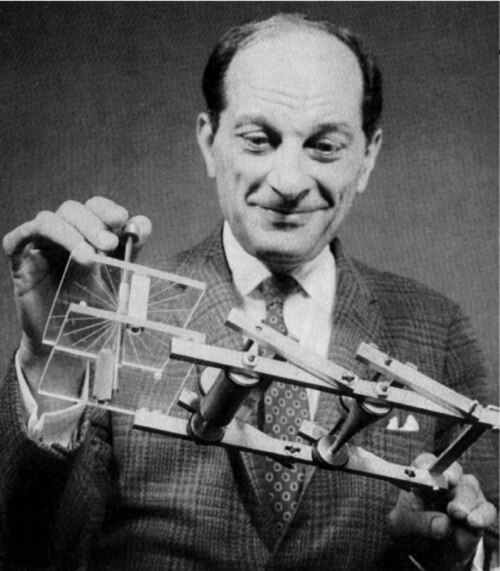
\includegraphics[width=\textwidth]{images/people/ulam.jpg}
        \caption{Stanisław Ulam e il FERMIAC.}
        \label{fig:ulam}
    \end{subfigure}
    \hfill
    \begin{subfigure}[b]{0.36\textwidth}
        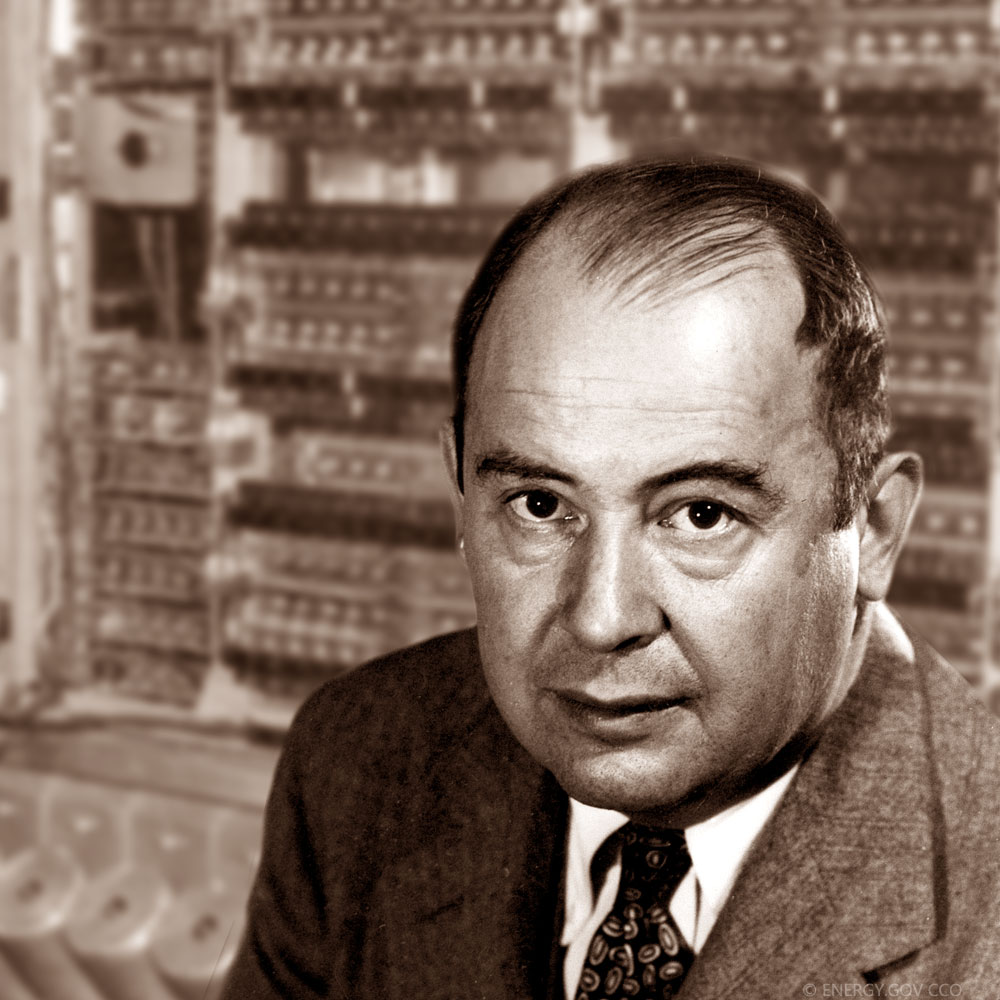
\includegraphics[width=\textwidth]{images/people/Von-Neumann-1000.jpg}
        \caption{Von Neumann.}
        \label{fig:von-neumann}
    \end{subfigure}
    \hfill
    \begin{subfigure}[b]{0.29\textwidth}
        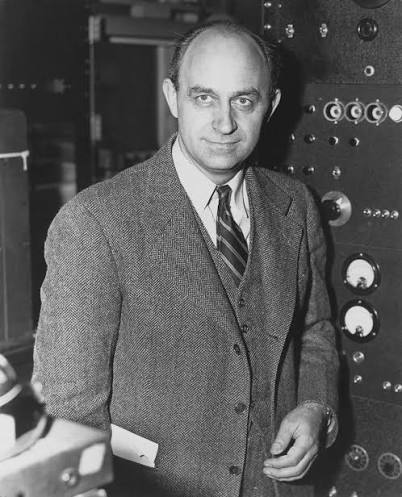
\includegraphics[width=\textwidth]{images/people/fermi.jpg}
        \caption{Enrico Fermi.}
        \label{fig:fermi}
    \end{subfigure}
    \caption{I pionieri del metodo Monte Carlo.}
    \label{fig:pionieri-mc}
\end{figure}

\section{Monte Carlo classico}
\label{sec:monte-carlo-classico}

\subsection{Metodo dell'inversa}
...

\section{Markov Chain Monte Carlo}
\label{sec:mcmc}
\subsection{Catene di Markov}

Sia ${X_1,..., X_N}$ una sequenza di variabili aleatorie in $\mathbb{R}^D$, questa sequenza è una catena di Markov se la probabilità condizionata di ogni $X_i$ soddisfa:

\begin{equation}
P(X_i |X_{i-1},..., X_{1}) = P(X_i | X_{i-1}).
\end{equation}

Dunque la probabilità di ottenere un certo valore di $X_i$ dipende solo dalla variabile aleatoria precedente della catena e non dalle altre, questa richiesta equivale a dire che la catena di Markov sono catene \textit{senza memoria}, ovvero che solo l'ultimo stato della catena influenza il prossimo stato \cite{quantum_monte_carlo_methods}. 
Considerando il caso che la variabile aleatoria $X_i$ possa assumere un numero discreto di valori, ovvero che $X_i \in \{x_1, ..., x_j, ...\}$, in questo modo possiamo descrivere la distribuzione di probabilità e le probabilità condizionate di tali variabili utilizzando un vettore e una matrice rispettivamente:
\begin{equation}
P(X_i) = p^{(i)}_j = \begin{pmatrix} p^{(i)}(x_1) \\ \vdots \\ p^{(i)}(x_j) \\ \vdots \end{pmatrix}, 
\quad
P(X_j|X_i) = P_{ij} = 
\begin{pmatrix}
P(x_1|x_1)  & \cdots & P(x_j|x_1) & \cdots \\
P(x_1|x_2) & \cdots & P(x_j|x_2) & \cdots \\
\vdots & \ddots & \vdots & \\
P(x_1|x_i) & \cdots & P(x_j|x_i) & \cdots \\
\vdots   & \vdots & \ddots
\end{pmatrix}
\end{equation}

Dove è possibile notare che le quantità $P_{ij}$, non dipendono dalle variabili nella sequenza che stiamo utilizzando grazie alle proprietà markoviane della catena. Inoltre possiamo notare alcune proprietà interessanti sia per $p^{(i)}_j$ che per $P_{ij}$, in quanto $\forall i$ esse soddisfano:
\begin{equation}
\sum_{j} p^{(i)}_j = 1, \quad \sum_{j} P_{ij} =1.
\label{ev_prob}
\end{equation}

Una catena di Markov è definita da una probabilità iniziale $p^{(0)}_i$ e da una matrice stocastica $P_{ij}$ detta \textbf{matrice di transizione}, poichè essa permette di generare la catena in modo ricorsivo:
\begin{equation}
    p^{(k+1)}_i = \sum_{j} P_{ij} p^{(k)}_j  \ \text{con } k \in \mathbb{N}.
\end{equation}

Questa evoluzione della distribuzione di probabilità della catena conserva la normalizzazione della distribuzione, infatti:
\begin{equation}
\sum_{i} p^{(k+1)}_i = \sum_{i} \sum_{j} P_{ij} p^{(k)}_j = \sum_{j} p^{(k)}_j \sum_{i} P_{ij} = \sum_{j} p^{(k)}_j = 1.
\end{equation}

Inoltre considerando una matrice di transizione ergodica(ovvero irriducibile e aperiodica) è assicurato che a prescindere dalla distribuzione iniziale $p^{(0)}_i$ iterando il procedimento si raggiunge una \textbf{distribuzione stazionaria} $p_i$ tale che:
\begin{equation}
    p_i = \sum_{j} P_{ij} p_j.
\end{equation}
Ovvero si raggiunge una distribuzione di probabilità che non viene più modificata iterando il procedimento (per questo detta stazionaria), inoltre essa è l'autovettore della matrice di transizione $P_{ij}$ con autovalore unitario.
L'obbiettivo di Markov Chain Monte Carlo è quello di costruire una catena di Markov che abbia come distribuzione stazionaria la distribuzione target $p_i$ che vogliamo campionare. Per fare ciò è necessario costruire una matrice di transizione $P_{ij}$ costruita in un certo modo. 

Metropolis et al. (1953) proposero che fosse possibile ottenere una specifica distribuzione $p_i$ se la $P_{ij}$ soddisfa una certa condizione di simmetria detta \textbf{bilancio dettagliato}: 
\begin{equation}
    P_{ij} p_j = P_{ji} p_i.
\end{equation}
Nella sezione successiva verrà presentato l'algoritmo di Metropolis, che permette di costruire una matrice di transizione $P_{ij}$ che soddisfa la condizione di bilancio dettagliato permettendo di campionare una distribuzione target $p_i$.

\subsection{Algoritmo di Metropolis}

Dunque per poter calcolare le quantità termodinamiche di interesse è necessaria una matrice di transizione che soddisfi il bilancio dettagliato per la distribuzione di Boltzmann.

Metropolis et al. proposero di costruire la matrice di transizione $P_{ij}$ come prodotto di due matrici:

\begin{equation}
P_{ij}=T_{ij}A_{ij},
\end{equation}
dove $T_{ij}$ è la matrice di proposta, che rappresenta la probabilità di proporre una transizione dallo stato $j$ allo stato $i$, e $A_{ij}$ è la matrice di accettazione, che rappresenta la probabilità di accettare la transizione proposta. Gli elementi della matrice di proposta $T_{ij}$ devono soddisfare le seguenti condizioni:
\begin{equation}
T_{ij} \ge 0, \quad \sum_{i} T_{ij} = 1 \quad \forall j, \quad T_{ij} = T_{ji}.
\end{equation}
Mentre gli elementi della matrice di accettazione $A_{ij}$ sono costruiti in modo che:
\begin{equation}
    A_{ij} = \min\left(1, \frac{p_i}{p_j}\right).
\end{equation}
Queste condizioni assicurando che la matrice di transizione rispetti il bilancio dettagliato, e quindi che la distribuzione stazionaria della catena di Markov sia la distribuzione target $p_i$, infatti (assumendo $p_i \le p_j$ senza perdita di generalità):
\begin{equation}
 P_{ij} = T_{ij}A_{ij} = T_{ji} \frac{p_i}{p_j} = P_{ji} \frac{p_i}{p_j} \implies P_{ij} p_j = P_{ji} p_i.
\end{equation}
L'algoritmo di Metropolis è quindi un metodo per costruire una catena di Markov che campiona una distribuzione target $p_i$ senza la necessità di conoscere la costante di normalizzazione della distribuzione, il seguente pseudocodice descrive l'operazione base dell'algoritmo di Metropolis:
\\
\newline
\begin{algorithm}[H]
\SetAlgoLined
\KwIn{Configurazione $X^{(i)}$; distribuzione target $p(x)$ nota a meno della costante di normalizzazione; distribuzione di proposta simmetrica $T$.}
    Genera uno stato proposto $X' \sim T(X^{(k)})$\;

    Calcola la probabilità di accettazione \ \ $ A=\min (1,\frac{p(X')}{p(X^{(k)})}); $

    Genera $u\sim\mathcal U(0,1)$\;

    \eIf{$u\le A$}{
        \Return $X'$\;
    }{
        \Return $X^{(i)}$\;
    }
\KwOut{Configurazione $X^{(i+1)}$.}
\caption{Operazione base dell'algoritmo di Metropolis}
\label{alg:metropolis}
\end{algorithm}
\vspace{5mm}
L'iterazione di questa operazione è l'algoritmo di Metropolis, che è possibile vedere rappresentato graficamente in figura \ref{fig:metropolis}, dove si osservano i passi del camminatore randomico, una distribuzione proposta (prior), una distribuzione target (posterior) e i campioni generati dal metodo.

\begin{figure}[H]
    \centering
    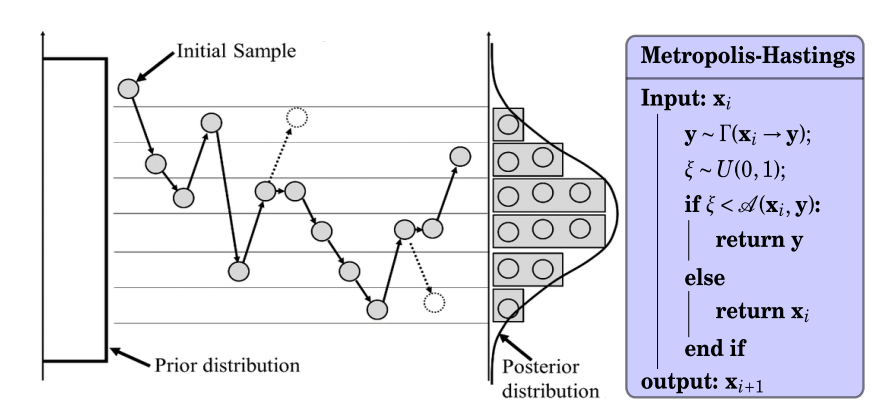
\includegraphics[width=0.9\textwidth]{images/MCMC/mcmc_algo.png}
    \caption{}
    \label{fig:metropolis}
\end{figure}

Dalla definizione della matrice di accettazione $A_{ij}$ è possibile notare che gli elementi di $P_{ij}$ dipendano esclusivamente dal rapporto della probabilità target nelle due configurzioni considerate (attuale e proposta), dunque sono indipendenti dalla costante di normalizzazione della distribuzione target. Come già espresso nel capitolo precedente, questo è un aspetto cruciale per il campionamento della distribuzione di Boltzmann, in quanto la costante di normalizzazione della distribuzione è proprio la funzione di partizione, di cui non è sempre possibile da calcolare analiticamente o numericamente.

Infine l'algoritmo di Metropolis trasferisce la responsabilità dell'ergodicità di $P_{ij}$ alla matrice $T_{ij}$. Se in un numero finito di passi $T_{ij}$ permette di raggiungere tutto lo spazio delle fasi, allora l'algoritmo di Metropolis è ergodico. Questo è un aspetto cruciale per il corretto funzionamento dell'algoritmo, in quanto la catena di Markov deve essere in grado di esplorare tutto lo spazio delle configurazioni per garantire che la distribuzione stazionaria sia effettivamente raggiunta. In altre parole, se la matrice di proposta $T_{ij}$ non consente di visitare tutte le configurazioni possibili, l'algoritmo potrebbe rimanere intrappolato in una regione dello spazio delle fasi, portando a stime errate delle quantità termodinamiche.
\section{Campioni autocorrelati}
\label{sec:campioni-autocorrelati}

\subsection{Blocking Analysis}

\subsection{Metodo di Sokal}